\section{Integración y funcionamiento.}

\begin{frame}{Conexiones utilizadas}

    Los códigos implementados en el ESP32 se encuentran en el repositorio de GitHub citado en \cite{Santana2025GitHub}, donde se indican las tres librerias principales \textbf{"lib\_encoder"}, \textbf{"lib\_stepperMotor"} y \textbf{"lib\_LCD"}.
    
    \begin{columns}[c]
        \column{0.5\textwidth}
            \begin{block}{Encoder}
                \begin{figure}[H]
                    \centering
                    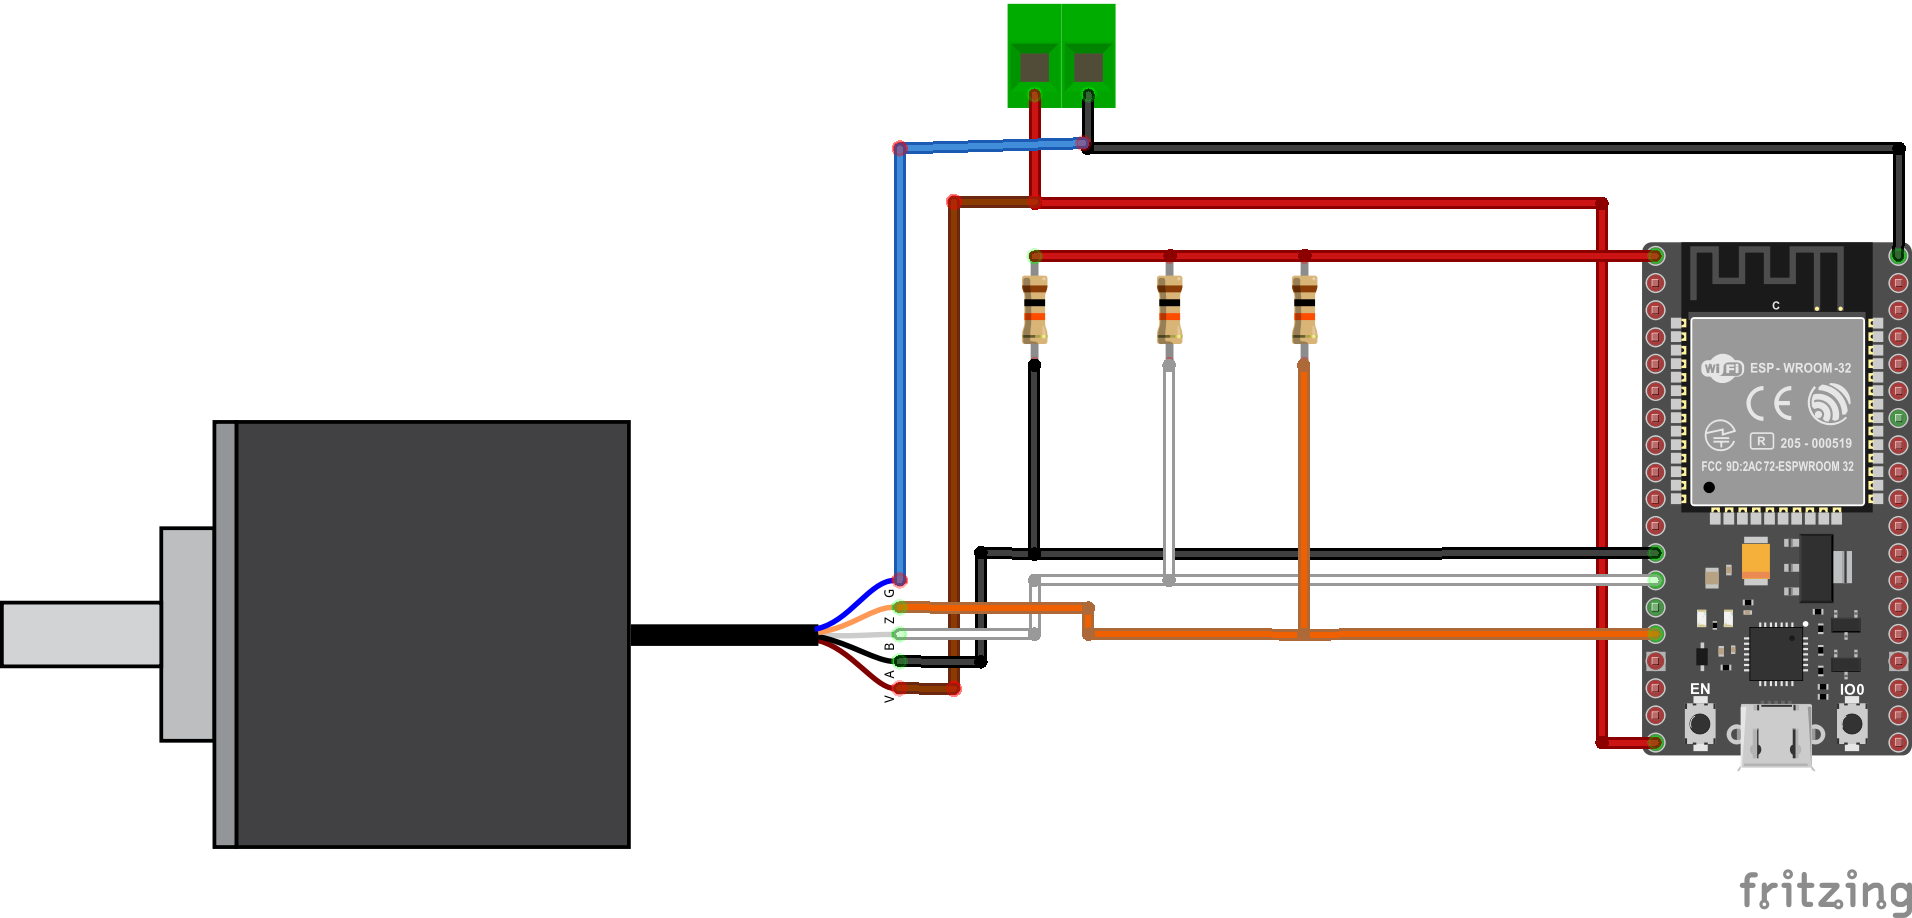
\includegraphics[width=\textwidth]{fig/diagrama_conexion_encoder_bb.png}
                    \caption{Diagrama de conexiones de integración encoder y esp32.}
                \end{figure}
            \end{block}
        
        \column{0.5\textwidth}
            \begin{exampleblock}{Motor y driver}
                \begin{figure}[H]
                    \centering
                    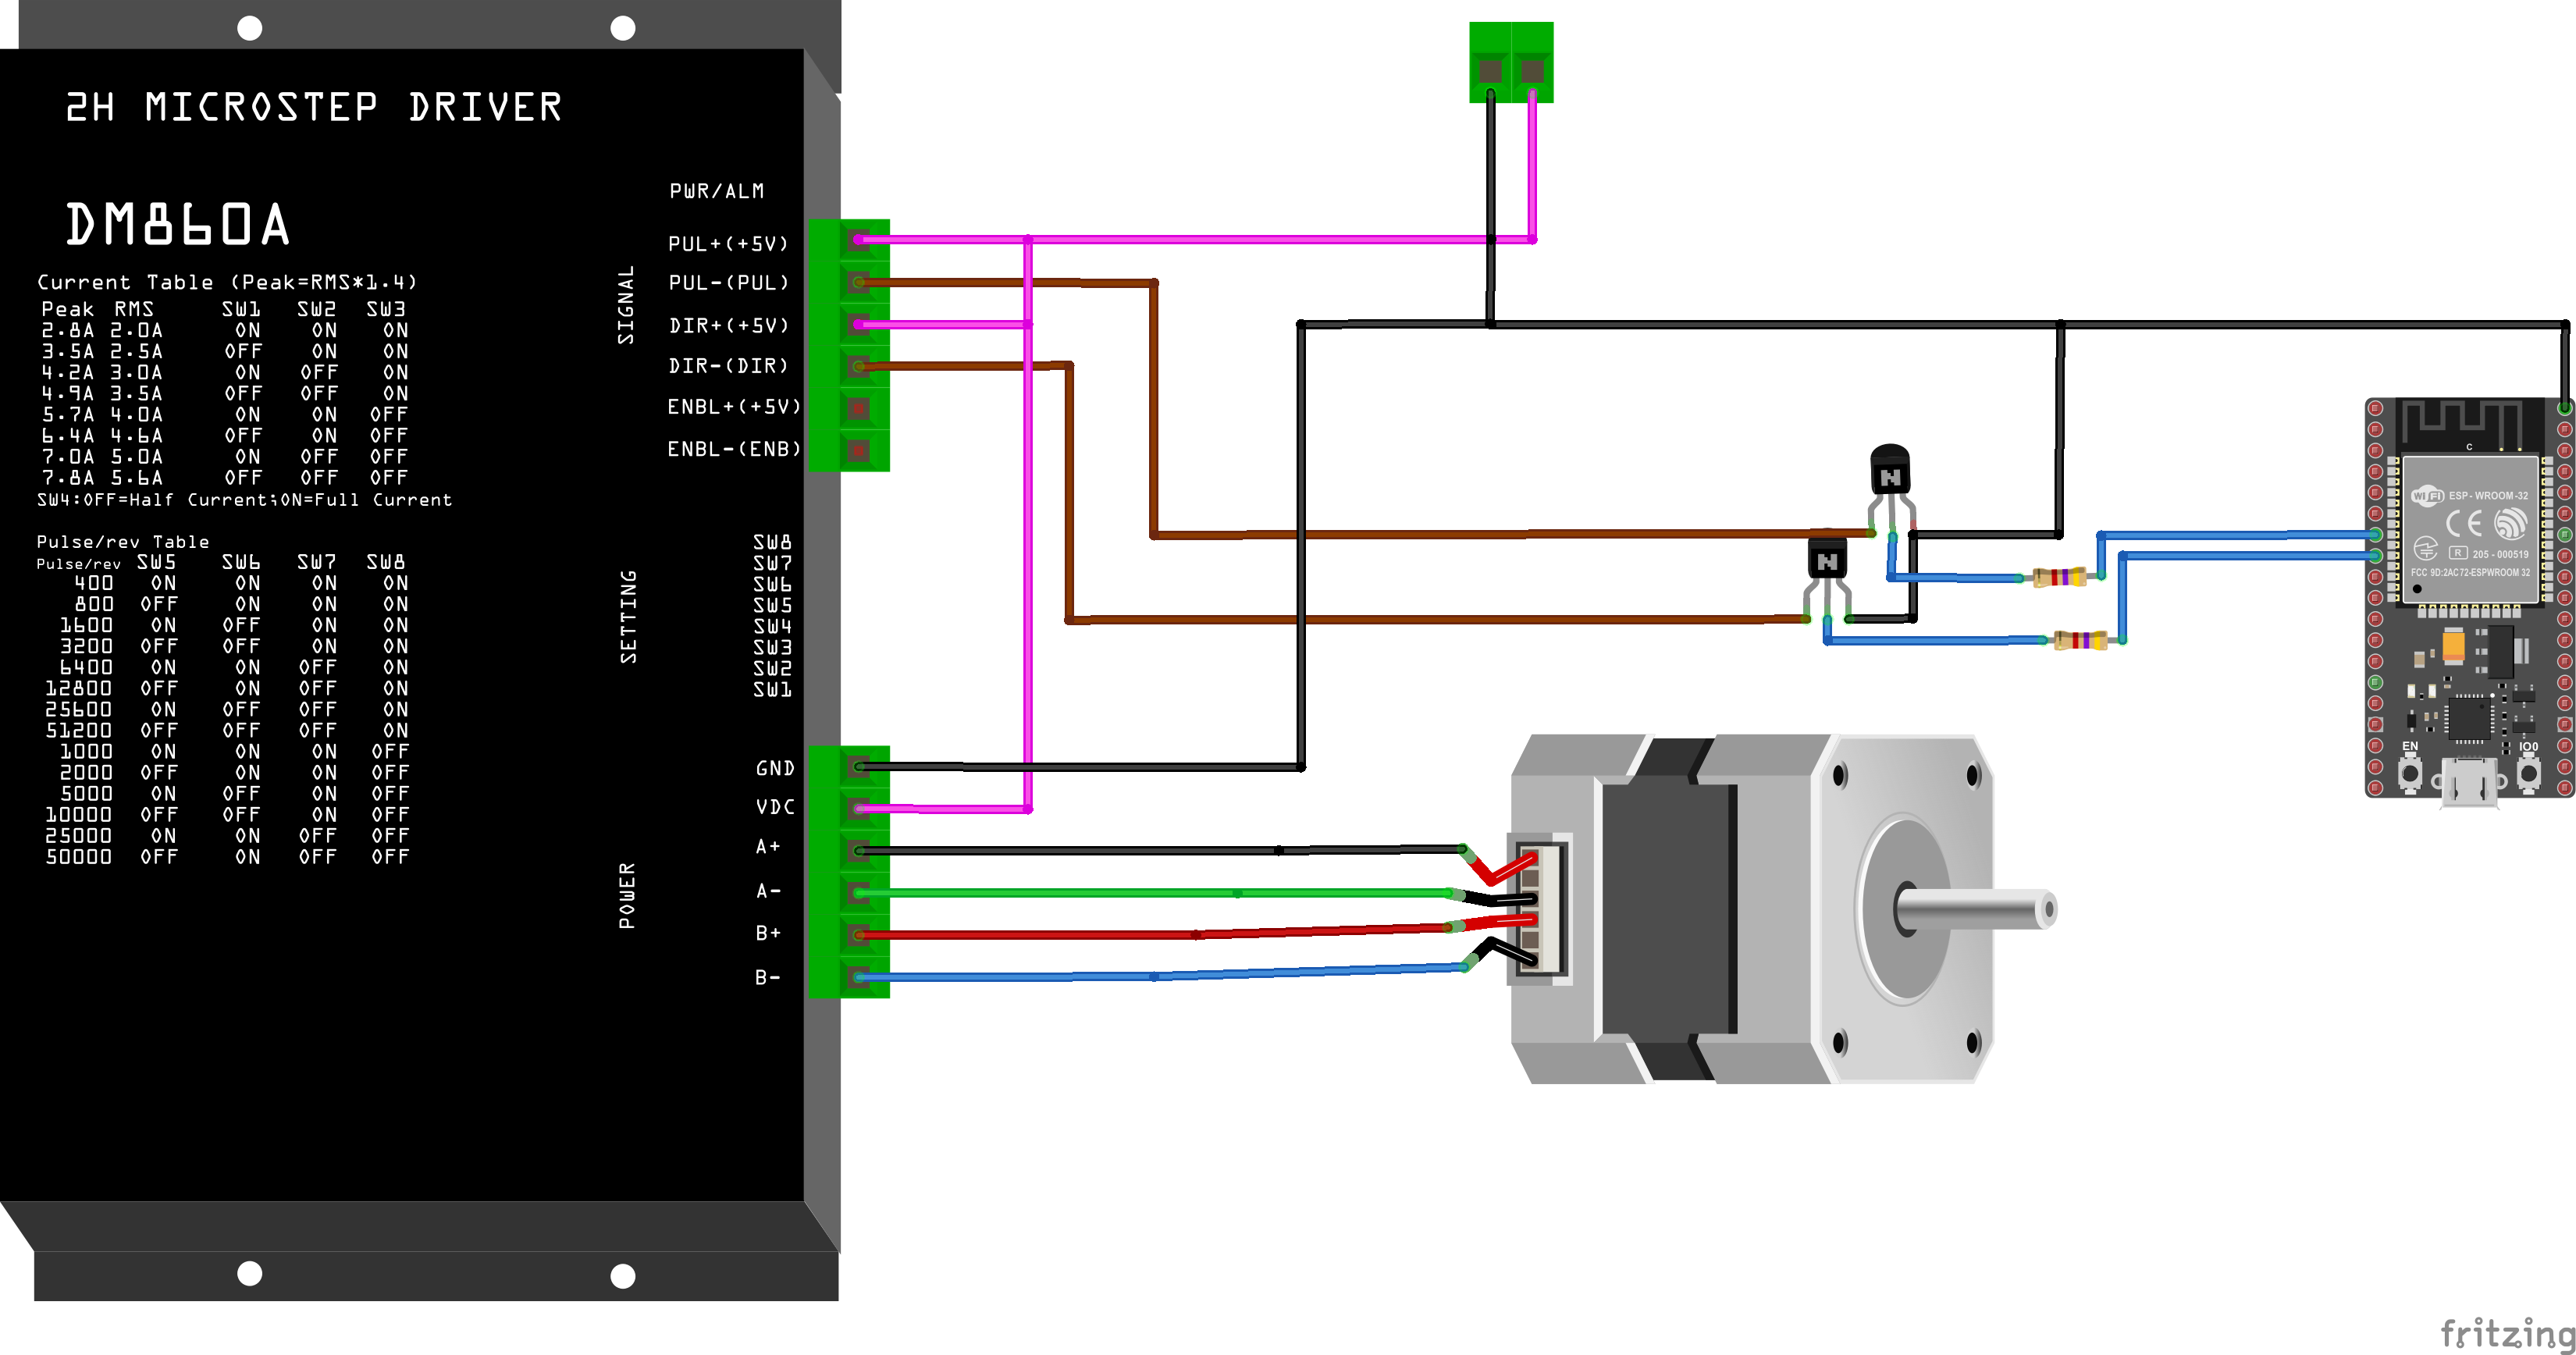
\includegraphics[width=\textwidth]{fig/diagrama_conexion_motor_bb.png}
                    \caption{Diagrama de conexiones driver y motor, en conjunto con el esp32.}
                \end{figure}
            \end{exampleblock}
              
    \end{columns}

\end{frame}

\begin{frame}{Diagrama de conexiones del sistema integrado.}

    \begin{figure}[H]
        \centering
        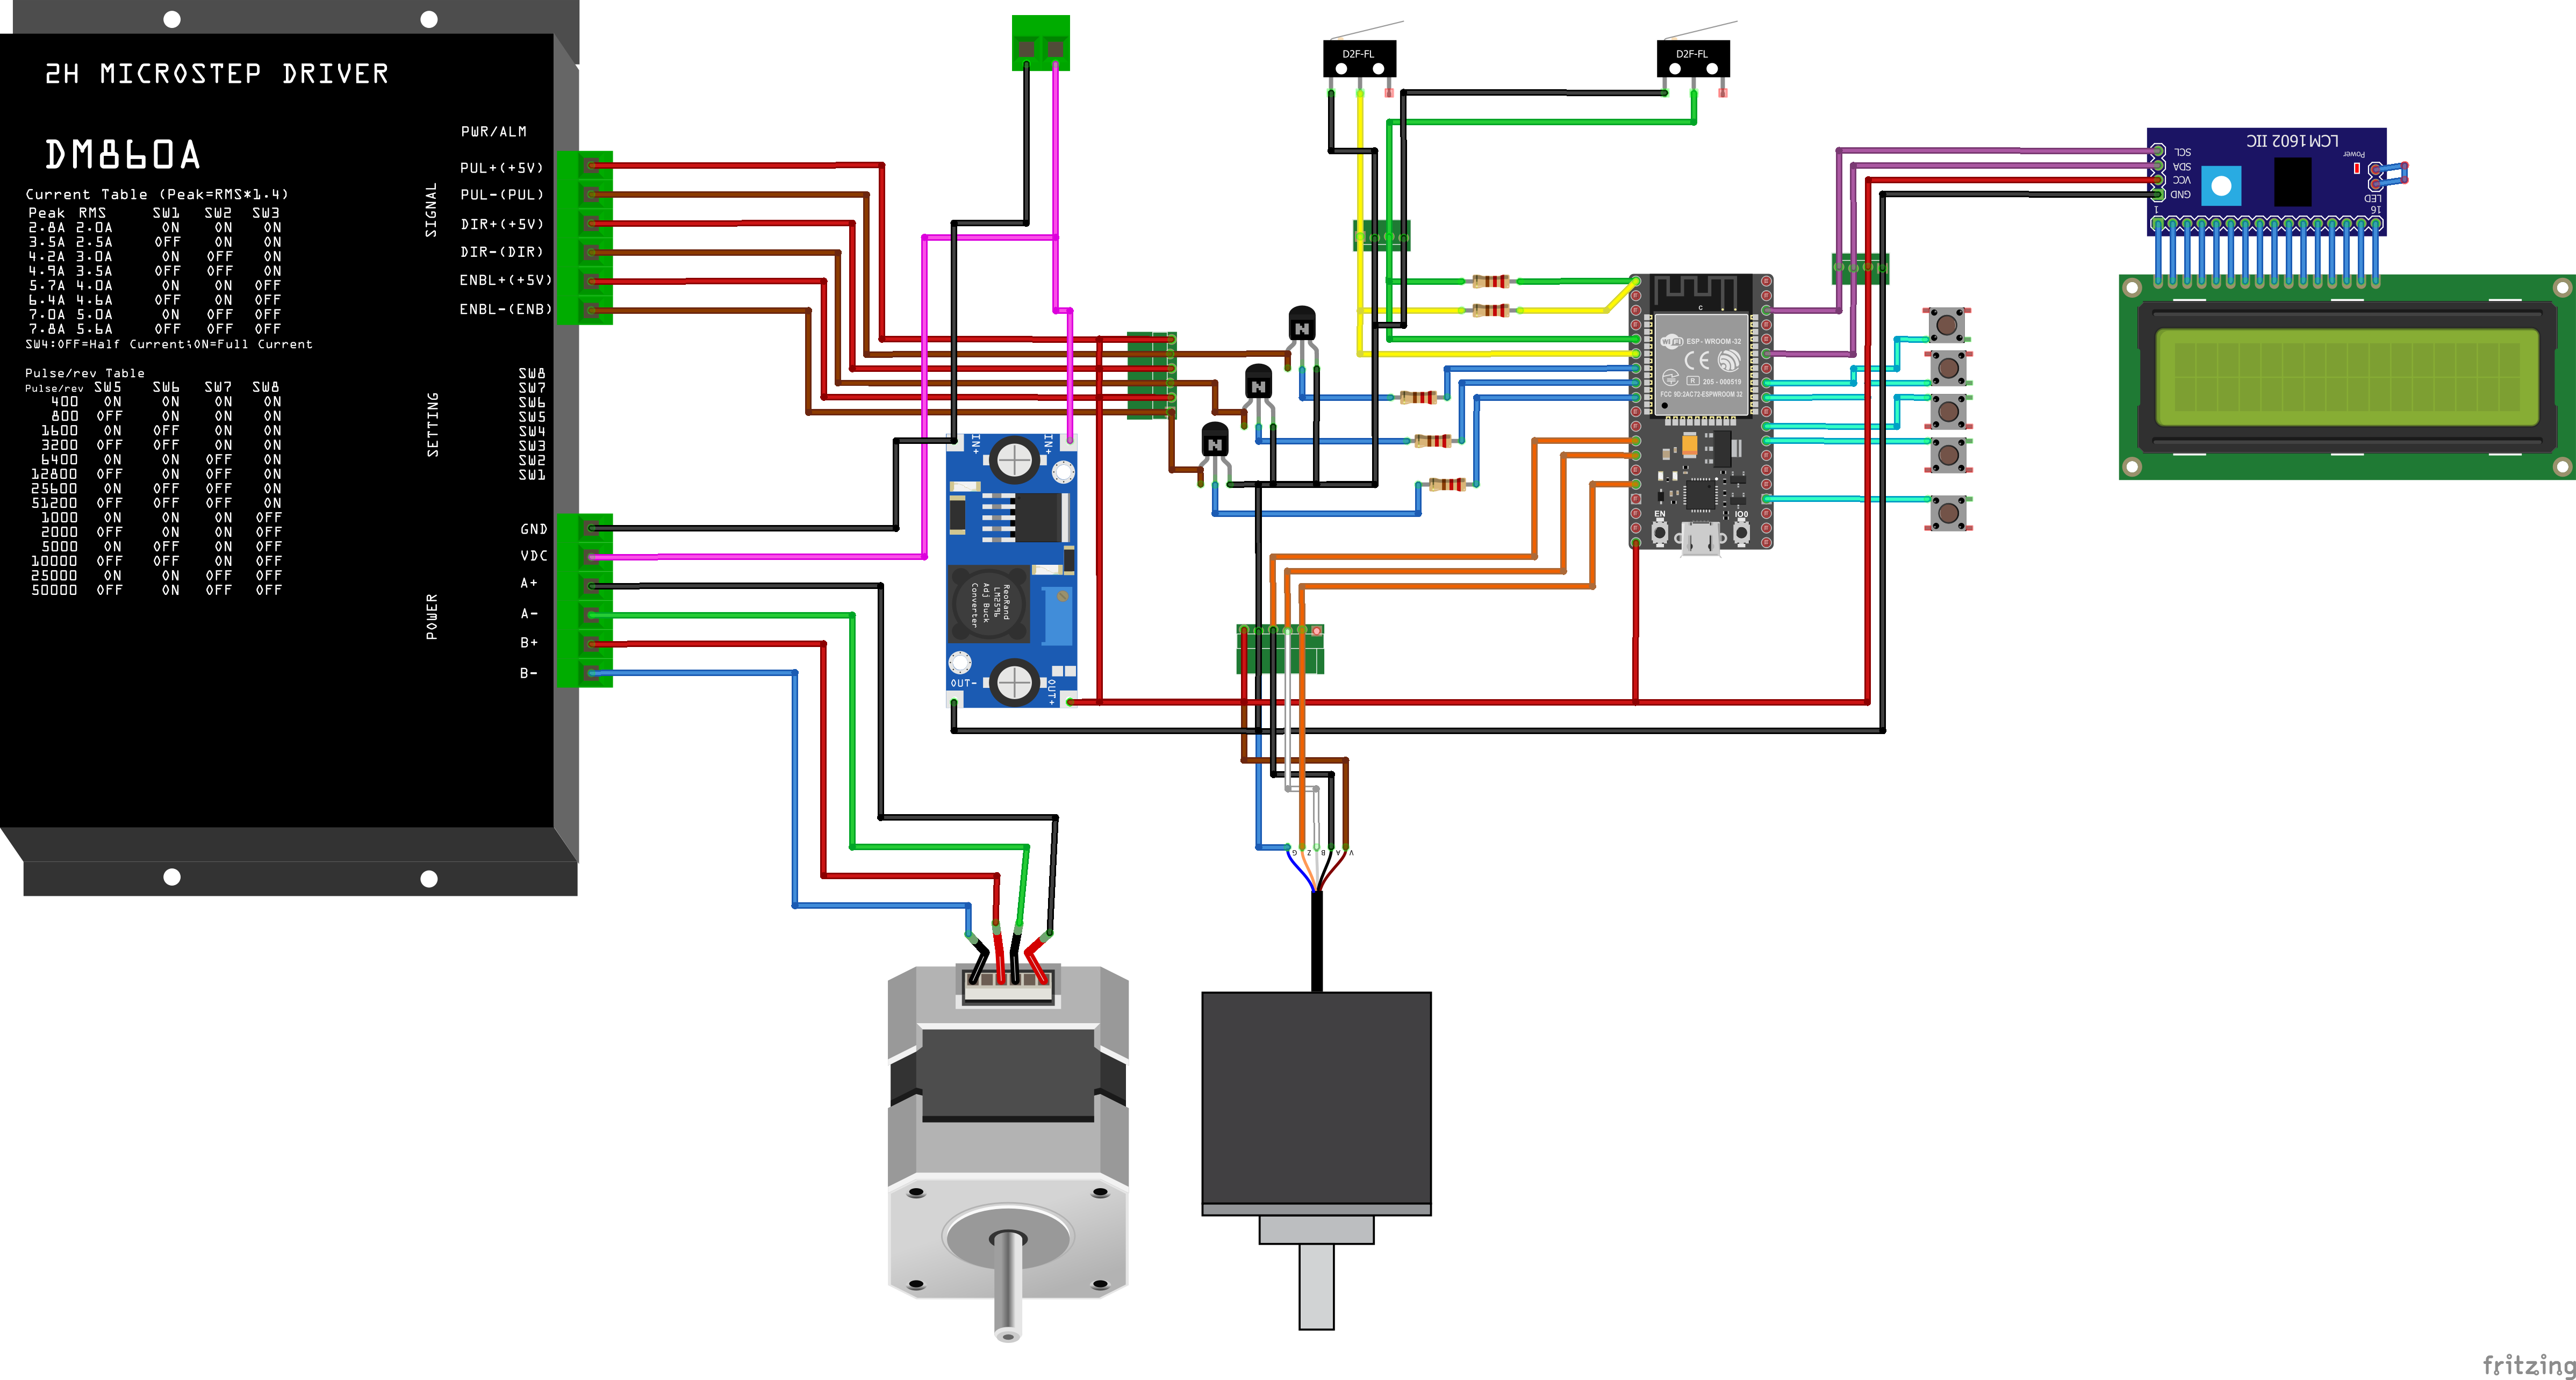
\includegraphics[width=0.9\textwidth]{fig/diagrama_conexion_control_bb.png}
        %\caption{Diagrama de conexiones de sistema.}
    \end{figure}

\end{frame}